\documentclass[12pt]{article}


\usepackage[numbers]{natbib}
\usepackage{graphicx} 
\usepackage{amssymb, amsmath, amsthm} 
\usepackage{fontenc} 
\usepackage{amscd,latexsym,amsfonts,amstext,amsbsy}
\usepackage{euscript} 
\usepackage{enumerate} 
\usepackage{color}  
\usepackage{physics}
\usepackage[latin1]{inputenc}
\usepackage{tikz}
\usepackage{mathrsfs}
\usetikzlibrary{shapes,arrows}
\usepackage{multicol}
\usepackage{comment}
\usepackage{color,soul}
\usepackage{combelow}
\bibliographystyle{apa}
\definecolor{applegreen}{rgb}{0.55, 0.71, 0.0}




\textwidth = 16 cm
\textheight = 24 cm
\oddsidemargin = 0.0 cm
\evensidemargin = 0.0 cm
\topmargin = -2 cm
\parskip = 0.2in
\parindent = 0.0in


\newtheorem{theorem}{Theorem}
\newtheorem{problem}[theorem]{Problem}
\newtheorem{exercise}[theorem]{Exercise}
\newtheorem{corollary}[theorem]{Corollary}
\newtheorem{lemma}[theorem]{Lemma}
\newtheorem{proposition}[theorem]{Proposition}
\newtheorem{proporties}[theorem]{Proporties}
\newtheorem{definition}[theorem]{Definition}
\newtheorem{definitions}[theorem]{Definitions}
\newtheorem{example}[theorem]{Example}
\newtheorem{remark}[theorem]{Remark}

 


\begin{document}
\textbf{``Modeling the Heroin Epidemic"} \\
Tricia Phillips \\
\today \\


%%%%%%%%%%%%%%%%%%%
%%%%%%%%%%%%%%%%%%%
%BACKGROUND%
%%%%%%%%%%%%%%%%%%%
%%%%%%%%%%%%%%%%%%%
\textbf{Background} \\
%Go back through and make sure everything from original source. If need more background, can always look at references in the background sections of many of the papers to get more paper ideas. 
\textcolor{green}{Heroin information} \\
%Heroin basic history: https://www.therecoveryvillage.com/heroin-addiction/heroin-facts-history/#gref AND http://www.unodc.org/unodc/en/data-and-analysis/bulletin/bulletin_1953-01-01_2_page004.html
Heroin is an illicit drug classified as an opioid and comes in the form of a white or brown powder or as a black substance resembling roofing tar. The drug is injected, sniffed, snorted or smoked and quickly enters the brain to bind to opioid receptors. It provides the user with feelings of euphoria, in addition to physical effects such as heavy feelings in the arms and legs, dry mouth, and sometimes nausea and vomiting \cite{NIH1, NIDA2}. There are short and long term negative effects on the body for using the drug, and consequently, it is currently considered a schedule I drug, meaning that there is no approved medical use of heroin and there is a high likelihood for abuse. \cite{DEA1, NIH1}. Addicted individuals have withdrawal symptoms such as restlessness, diarrhea, vomiting, and cold flashes, along with cravings for the drug which makes stopping use of the drop very difficult \cite{NIH1}. Options for treatment for heroin use involve medications such as buprenorphine, methadone, and naltrexone, in combination with counseling and behavioral therapies \cite{SAMSHA1, NIH1}. Heroin users build up a tolerance to the drug with repeated use and can overdose on the drug, in which their heart rate and breathing is slowed to a dangerous level without medical assistance \cite{NIDA2, NIH1}. Due to built-up tolerance, the risk of overdose is high when individuals stop their use of the drug for a period of time (i.e. while in recovery or hospitalized) and return to use. This is because they may return to the previous amount they were taking before, without knowing what their body can currently tolerate \cite{NIH2}.  

A national survey estimated that out of the United States national population of individuals 12 years of ago or older, 948,000 were heroin users in 2016, although this number may include under-reporting \cite{CDC2}. There were an estimated 13,219 heroin deaths in 2016, a more than six-fold increase from the year 2002, despite there being roughly half as many heroin users in 2002 \cite{NSDUH1}. This, in part, is due to the recent trend of lacing heroin with fentanyl, a surgical-grade opioid that is up to fifty times more potent than heroin alone, and therefore, users are unaware of the purity of the heroin they obtain \cite{CDC1, NIH2, Volkow2}. The effects of heroin, however, extend further than just the using individual. Due to the sharing of needles and other equipment involved in the injection of heroin, the human immunodeficiency virus (HIV) and the hepatitis C virus (HCV) are more easily contracted as transmittance occurs through bodily fluids. Moreover, risky sexual behavior is more likely under the influence, so for those whose method of use is via smoking or snorting, there is also an increased risk of transmitting and contracting these viruses. Women who use heroin during pregnancy put their babies at risk for neonatal abstinence syndrome in which the drug is passed along to the baby, resulting in dependency and thus, withdrawal symptoms upon birth \cite{NIDA2}. 

Heroin was first formulated in a hospital in 1874, but production on a commercial level did not begin until 1898, when the Bayer Company in Germany marketed and sold the new drug. Prescription heroin was deemed helpful for treating bronchitis, asthma and tuberculosis, but near the turn of the century, the dangers of the drug were starting to be revealed, such as it's potential for addiction. In 1920, the American Medical Association stated that heroin should not be manufactured, sold, or prescribed in the United States, and in combination with the amount of crime resulting from heroin use, a law was passed in 1924 prohibiting crude opium imports with the intention of heroin production. With the start of World War II, traffickers diluted the drug more and more, due to tighter border controls and fewer supplies entering the country \cite{UnitedNations}. \textcolor{red}{More heroin history: find reliable source for smuggling of heroin from China to US in 1930s; motor vehicle vs. drug overdose stats; ~750,000 heroin addicts from 1965-1970; purity level/price of heroin; provide argument for why the problem is so large now that we need data-driven models compared to just a theoretical heroin addiction model as done for decades.} 

%Egan paper made a good point that even though the number of individuals going into treatment has increased, that does not mean more users necessarily, could mean more treatment facilities opened up/spots available 
\textcolor{green}{Fentanyl information} \\
\textcolor{red}{Put in background on fentanyl.} \\

\textcolor{green}{Prescription opioid information} \\
Another large portion of opioids consist of prescription pain relievers which are either natural, such as morphine and codeine, semi-synthetic, such as oxycodone, hydrocodone, and oxymorphone, or synthetic, such as fentanyl and tramadol \cite{CDC3, TNMentalHealth2}. From 1991 to 2011, there was a near tripling of prescriptions that pharmacies distributed \cite{NIDA1}. This was in part due to a number of new opioids that were approved by the FDA for use, such as OxyContin, Actiq, Fentora, and Onsolis (fentanyl), in addition to other unapproved opioid products for pain management \cite{FDA1}. Moreover, in the early 2000s, drug manufacturers funded publications and physicians to support opioid use for pain control \cite{Mandell}. A national survey estimated there were 11.5 million individuals 12 years of age or older in the United States that experienced pain reliever misuse in the past year, referring to the year 2016 \cite{CDC2}. In this survey, misuse was defined as taking the prescription at a higher dose, more frequently or longer than prescribed, taking someone else's medication, or any other way not directed by a doctor \cite{SAMSHA3}. This subset of the opioid drug class is misused for a variety of reasons and the same survey asked individuals who reported prescription pain reliever misuse to give the reason and the source for their most recent misuse. The most prominent responses for reasons of misuse were to relieve physical pain, to feel good or get high, and to relax or relieve tension. The largest source was from friends/relatives or from a healthcare provider, followed by given a prescription or stolen from a health care provider \cite{CDC2}. Treatment options for opioid addiction are the same as heroin \cite{SAMSHA1}. In addition, pregnant women who take prescription opioids also put their babies at risk of neonatal abstinence syndrome, similar to heroin \cite{CDC5}. 

\textcolor{blue}{Question: Maybe leave out since so prescription focused?}: In 1995, the American Pain Society stated that pain was being under-treated in doctor offices and hospitals, and consequently, created guidelines for the improvement for pain assessment for acute and cancer cases. This included the recording of pain levels such as on a vital signs sheet \cite{Mandell, APSQCC}. In 2000, the Joint Commission required physicians to accept and respect the self-reporting of pain by patients. By the early 2000s, drug manufacturers funded publications and physicians to support opioid use for pain control \cite{Mandell}.  

\textcolor{green}{Connection between opioid and heroin abuse} \\
The misuse of prescription pain relievers leads some individuals to start heroin. %Find source that talks about having similar pharmalogic properties (one of the government websites, I think) 
According to the National Survey of Drug Use and Health (NSDUH) survey information from 2002-2011, nearly 80\% of heroin users reported non-medical prescription pain reliever use prior to their heroin use. Here, non-medical prescription use is defined as taking prescriptions that were not prescribed to the user directly or used only for the feelings it causes. In fact, those who had prior non-medical prescription pain reliever use were 19 times more likely to initiate heroin use than those without prior use \cite{Muhuri}. This could in part be due to the higher availability of heroin in recent years at a lower cost than alternative opioids \cite{NIDA1}. Moreover, approximately 3.6 percent of non-medical prescription pain reliever users began using heroin within 5 years of their first opioid; although a small percentage, this is a significant number of individuals given the magnitude of opioid addiction \cite{Muhuri}. In 2010, an abuse-deterrent formulation of the commonly abused prescription opioid OxyContin was released that made abuse through injection and inhalation more challenging. Although done with the intent of reducing opioid abuse, studies showed that many individuals switched to heroin use instead \cite{Cicero2, Cicero3}. One study of young adults ages 18-25 concluded that among many factors including race, education status, martial status, other drug use, as well as many others, the use of non-prescribed opioid pain relievers in the past year was the biggest indicator of an individual using heroin in the past month, past year or in their lifetime \cite{Ihongbe}. Comparing NSDUH data from 2002-2004 and 2008-2010, the average yearly rates of past year heroin use increased among non-medical opioid users, but heroin use stayed static for those who reported no non-medical use of opioids; the highest rate of heroin use was among individuals with past year non-medical use of opioids ranging between 100 and 365 days of use \cite{Jones}. 

\textcolor{red}{Add more in here from background papers.}\\ In the 1960's, heroin users were composed mainly of younger, nonwhite men in urban areas with their initial opioid being heroin, but in recent decades, this trend has shifted to older, white, rural and suburban men and women with their initial opioid being a prescription \cite{Cicero}. Opioids are of no shortage in society today and since opioid addiction is driven largely by legal prescription medication availability, this has made a significant proportion of society susceptible to misuse and addiction to opioids, including heroin. 
\textcolor{red}{Tennessee: TN Together Law (initial prescriptions have limit of 5 days with limited dosage of 40 morphine milligram equivalents, MME's), Pilfering Prevention Act (lockable bottles to reduce kids from getting access) and STOPTN (community group in TN). Great summary of statistics for Tennessee specifically: https://spark.adobe.com/page/mKMP4PaXOtIAy/}


\textcolor{green}{Goal paragraph} \\ 
The misuse of opioids, including prescription pain relievers, synthetic opioids, and the illegal drug heroin, is rampant in today's society \cite{NIH2}. The opioid crisis was declared a public health emergency in October 2017 by the United States Department of Health and Human Sciences \cite{HHS1}. It was estimated that the total economic cost of prescription opioid dependence, abuse and overdoses in 2013 alone was \$78.5 billion \cite{Florence}. Due to the health risks of the addicted individuals, public health concerns, the number of overdose deaths and the economic burden, this is an issue worth paying attention to.
To address this apparent problem in today's society, we wish to model the prescription opioid/heroin/fentanyl epidemic in order to understand the dynamics behind the epidemic and predict the trajectory of the epidemic. We also wish to identify important conditions relating to the reduction of opioid/heroin/fentanyl addiction. To do that, we have formulated a population level system of ordinary differential equations model consisting of classes of individuals taking prescription opioids, addicted to opioids, using heroin or fentanyl, and recovering from addiction to opioids, heroin and/or fentanyl, and analyzed it. Our overall goal is to explore how different management strategies may alter the epidemic trajectory; specifically, we would like to investigate management strategies for optimally treating pain with prescriptions while reducing opioid, heroin, and fentanyl addiction.

\textcolor{green}{Other models} \\
There have been several models formulated focusing on heroin addiction. Most of them were motivated by and extensions of the White and Comiskey ordinary differential equation model with three compartments each representing a different stage as a drug-user: the susceptible class including individuals aged 15-64, the drug user class composed of individuals not in treatment, and finally, the drug users in treatment. In this model, individuals in treatment for drug use were only able to die, relapse to drug use, or complete treatment and be immune to drug use for the remainder of the modeling time period. The basic reproduction number, $\mathscr{R}_0$, was calculated and deemed most sensitive to the rate of individuals in the susceptible class becoming drug users; therefore, prevention is more important than treatment for reducing drug use \cite{White}. Wang, Yang and Li did analysis of this model, changing the assumption that the population was not constant \cite{Wang}. 

%\textcolor{blue}{Question: How can the model assume the three compartments make up the entire population, but then have the option for immunity to drug addiction for the remainder of the modeling period? Answer: NOT necessarily the same people; just equal number of people (i.e. someone is born susceptible to replace someone who became immune, maybe)  

The White and Comiskey model was modified later on by Liu and Zhang in order to incorporate a relapse distribution in which there was a non-constant time to relapse. They formulated a delay-differential equation, and also took away the assumption that the population was constant. Their conclusions about the sensitivity of $\mathscr{R}_0$ to certain parameters were in line with those from White and Comiskey \cite{Liu}. Using the same three compartments, another model was formulated with the idea of the relapse rate relying on the length of time the individual has been undergoing treatment. This coupled ODE-PDE model assumed that susceptibles could only become addicted via interaction with heroin users not undergoing treatment. Prevention was deemed more important than treatment, yet again \cite{Fang1}. Fang, Li, Martcheva and Caialso (2015) also modeled the heroin epidemic allowing susceptibility of becoming a drug user to depend on age, again resulting in a coupled ODE-PDE model \cite{Fang2}. A non-autonomous version of the White and Comiskey model included a distributed time delay for becoming a drug user along with both the parameters and the total high-risk population size being time-dependent \cite{Samanta}. From this, an autonomous model was developed incorporating the distributed time delay, which was converted into a discrete model with the time step-size being one \cite{Abdurahman}. Finally, a three compartment model consisting of susceptibles, users not in treatment, and those in treatment, assumed that those not in treatment could not recover and return to being susceptible, and that it took two contacts with a drug user to become addicted, resulting in a nonlinear incidence rate; results showed that perhaps the heroin prevalence undergoes periodic changes depending on conditions \cite{Ma}. 
%\textcolor{blue}{Question: Should I go through each paper specifically, like I have above, or moreso "group them" by stating some ways that the White and Comiskey model was modified and then reference them all together?} Answer: do them individually, that's better 

A deviation from the three compartmental model was done that included a fourth compartment which consisted of individuals who successfully recovered from their heroin use, whether through deciding to stop use by themselves or via treatment measures. The treatment of heroin users is limited by the availability of treatment facilities and resources and therefore, a saturated treatment function is incorporated; the saturation parameter was concluded as having the most vital role in the persistence of the epidemic. This implies that intervention is important early on before heroin addicts accumulate in the community and thus, prompt treatment is necessary \cite{Wangari}. 
 %http://journals.plos.org/plosone/article/file?id=10.1371/journal.pone.0102263&type=printable) 
Another model consisting of 84 ODE's captured the dynamics between prescription opioid users with acute pain, those with chronic pain, illicit opioid users, heroin users and those who overdose. Results showed that increasing addiction treatment and reducing prescriptions for individuals with chronic pain seemed to have a greater impact on reducing both heroin overdose deaths and the number of opioid abusers compared to reducing prescriptions for acute pain without treatment increases \cite{Benneyan}. \textcolor{red}{This was from a conference preceding...in future, look for published model from Benneyan.} 

%\textcolor{blue}{Question: Should only include population level models, correct...not something like a heroin market model (agent-based) with drug users, sellers, homeless \& police?} Will put in that model, and can do anything related because if those authors are editors, they will not like if they don't see their own work referenced. 

Others have taken a completely different approach, specifically using agent-based modeling. In addition to their ODE model, Benneyan, Garrahan, Ilie\cb{s}, and Duan (2017) formulated two agent-based models: the first being a cellular automata model consisting of a grid with neighboring cells updated depending on state variables adjacent to the cells; the second being a network model with nodes that represent individuals/subpopulations and weighted pathways dependent on relational strength and nearness. \textcolor{red}{Not all variables are defined, such as P(x,y), so should I ask for full model from Benneyan?} The former was to better understand regional spread and the latter to investigate spread among individuals; their results suggested that with various regulation practices for opioids, heroin death rates would decrease, but the authors recognize the reality of unintended consequences of these legislations \cite{Benneyan}. Agar (2001) created an agent-based model, consisting of a world with 2,500 patches and 100 agents each assigned an experimentation value which defines how likely that individual is to experiment with heroin, depending on their interest in trying something new, their attitude toward illicit drug use, and their desire to follow societal rules. The model was able to track the number of heroin experimenting individuals over time with the agent moving randomly, one patch selected at random to contain heroin in the beginning, and the ability for individuals to obtain heroin from their original patch, from others who have experimented, or from another patch where the transferring of heroin between agents occurred \cite{Agar}.

\textcolor{red}{UPDATE with new revisions/any new results from version that was accepted!!} The motivation for our heroin model came from a previous model focusing on opioid addicts through prescriptions or via the black market \cite{Battista}. In order for the model to have an addiction-free equilibrium, both addictions that come from prescriptions and addictions from accessibility to excess prescription drugs must be eliminated, which equates to the need for close administration and monitoring of those prescribed. Furthermore, near the addiction-free state, the prevention of prescription opioid users becoming addicted is more important for staying near the addiction-free equilibrium than reducing the number of prescriptions getting into the hands of non-prescribed users. \textcolor{blue}{Question: any endemic equilibrium explicitly calculated or showing have forward bifurcation is enough for existence + endemic equilibrium connection or no to the AFE analysis?} However, away from the addiction-free state, a realistic situation, the most important factors in reducing the number of addicted individuals include increasing the prescription completion rate, increasing entry into treatment (even among low success rates), and decreasing the prescription rate. The purpose of formulating a separate model from this prescription opioid model is to be able to understand the more complicated dynamics that arise among opioid addiction with the addition of heroin use. As exemplified previously, heroin and fentanyl play a significant role in the process of opioid addiction and recovery and so it's inclusion provides a more accurate overall picture of the epidemic. In addition, since heroin users overdose almost as much as prescription opioid users and in recent years, a sharp increase of heroin overdoses has occurred primarily due to the involvement of fentanyl, it is crucial to take a more detailed look at this increasing problem \cite{CDC4}. 

\textcolor{red}{Put in brief explanation of ``Reducing the complexity of an agent-based local heroin market model" paper by Heard} 

\textcolor{red}{Look up if any models regarding fentanyl use/addiction.} \\

\textcolor{red}{Include details on how my model different than the previous ones.} For the most part, models have not incorporated the connection between prescription opioid misuse and heroin or fentanyl use at all, instead focusing solely on heroin addiction and recovery. Although there are many factors that play a role in population size, susceptibility to drug use, relapse time and other parts of the drug-using process, we consider individuals in each of the classes to be homogeneous, for simplicity of a starting model. 

%Compton says that current efforts from state and federal level: educating health professionals/public about appropriate use, prescription drug-monitoring programs, regulations about excessive prescribing (pill mills) and producing abuse-deterrent opioids 

\textcolor{orange}{Future models to look for when published: \\
``Sub-epidemics within the opioid epidemic" by Hawre Jalal, Jeanine Buchanich, Lauren Balmert, Mark S. Roberts, and Donald Burke (see notes in binder from 7/2018); \\ 
``Leveraging Geospatial Methods to Accurately Identify Clusters of Opioid Drug Abuse and Target Interventions" by Zan Dodson, Eun-hye Yoo, and Jeanine Buchanich; \\
``A Dynamic Disease Transmission Model of the Opioid Epidemic" by David Sinclair, Hawre Jalal, Mark S. Roberts, and Donald Burke; \\ 
``A Multi-Cohort Simulation Model of the Opioid Epidemic" by Hawre Jalal, Mark S. Roberts, and Don Burke \\
``Heroin math: the good, the bad and the ugly" by Nicholas Battista; \\
Statistical model, opioid natural history model, drug contagion model, and individual based simulation model (FRED concept) by Hawre Jalal from Pitt conference; \\
12 compartment model with 11 intervention scenarios by Margaret Brandeau from Pitt conference; \\
Compartmental model and community opioid agent-based model by Georgiy Bebashev from Pitt conference}

\textcolor{green}{Extensions}\\
In our model we assume homogeneous mixing of the individuals in each of the compartments and therefore, each individual has the same probability of transitioning from one stage to another, interacting with individuals from other stages, or leaving the system via death. Although done for the purpose of simplification, this is not an accurate representation of reality since there are factors that affect these probabilities, such as race, gender, geographical location and age. For example, there has been a shift in heroin use from urban areas to some suburban and rural areas and there is an increasing number of individuals ages 18-25 using the drug \cite{NIDA2}. West Virginia, New Hampshire and Ohio had the highest rates of opioid-related overdose deaths per 100,000 people in 2016 and Tennessee and Arkansas were among the states with the highest prescription rates per 100 people the same year \cite{NIH3}. Men have a higher likelihood of overdosing on prescription pain relievers compared to women, but since 1999, there has been a steeper increase in the number of women overdoses than men. In addition, women may form a quicker dependence on opioids compared to men, and have a higher probability of being prescribed higher doses and for longer periods of time \cite{CDC5}. Specific to heroin, using data from the 2008-2010 NSDUH studies, past year heroin use was twice as likely for men compared to women, and highest in the 18-25 year old age group \cite{Jones}. Incorporating these ideas into the model and parameter information would be possible future extensions. Although there is data on the misuse of opioids, we decided to focus specifically on addiction rather than misuse, due to the harmful consequences this behavior can have for an individual. However, the behavior and actions of individuals are not always very clearly defined, and there may be a benefit to expanding the spectrum of classes that individuals can fall into. 


%Great explanation of why model needed/how go about it: http://science.sciencemag.org/content/354/6312/529 

\textcolor{red}{In introduction of disseration, can write info from previous meetings/opioid sessions I've attended to share everything I've learned about the topic.}




%%%%%%%%%%%%%%%%%%%
%%%%%%%%%%%%%%%%%%%
%MODEL FORMULATION%
%%%%%%%%%%%%%%%%%%%
%%%%%%%%%%%%%%%%%%%



\textbf{Model Formulation} \\ \\
To the extent of our knowledge, there have been no mathematical models incorporating both prescription opioid use and heroin use. \textcolor{red}{Write up differences within my model compared to other models.}
Our model consists of five subgroups of the \textcolor{red}{(Tennessee)} population, in which they are all proportions of the entire population: 

1. Susceptibles ($S$): This portion of the population consists of individuals who are not taking prescription opioids of any kind, nor using heroin or fentanyl. \\ \\
2. Prescription opioid users ($P$): This class of individuals consists of individuals who are prescribed opioids by a health care provider and take the opioids at a level that is not considered addicted. We note that individuals in this class could be misusing prescription opioids, but not at the level of addiction.  \\ \\ %"Misuse" in data: questions may ask about misuse in the past 12 months, and so even 1 time of misuse would count 
3. Opioid addicts ($A$): This group of individuals are addicted to opioids, but not using heroin or fentanyl, or are actively in treatment for opioid addiction, or are within 4 weeks post-treatment for opioid addiction. (Although the opioid class of drug includes heroin and fentanyl, here we will take opioids to mean non-heroin and non-fentanyl.) \textcolor{red}{We assume very few, if any, individuals are addicted to opioids outside of prescription opioids, but even if they are, they are probably are taking prescription opioids anyways, so this is our reasoning for taking those with pain reliever use disorder as initial condition because already includes those with other non-prescription opioid addiction} \\ \\
\textcolor{red}{I believe ROSIE study says somewhere that individuals in treatment are mostly still taking drugs, which supports our decision to leave those in treatment in an addicted class: https://www.drugsandalcohol.ie/11542/1/ROSIE3-YearReport.pdf} \\
4. Heroin/fentanyl users ($H$): This class is composed of individuals who are addicted to heroin or fentanyl or are actively in treatment for heroin/fentanyl addiction, or are within 4 weeks post-treatment for heroin/fentanyl addiction. We note that individuals in this class could be using other drugs or are addicted to opioids in addition to heroin or fentanyl, but they are at least addicted to one of these drugs. \\ \\
5. Recovered individuals ($R$): This class consists of individuals who completed treatment for opioid or heroin/fentanyl addiction and did not relapse within 4 weeks post-treatment, and therefore are considered in a ``stable/successful" state of being recovered. We make assumption that those in the recovery class are not considered addicted.


We assume that these five compartments sum to one, so that the population is of constant size, i.e. the total death rate is equal to the incoming rate for the susceptible class. Although terminology is not always clearly defined in the literature, such as opioid misuse, abuse, dependency, addiction and use disorder, we aim to focus on addiction only, where addiction to opioids is defined as having a pattern of continued non-medical use that is already, or could be, harmful \cite{Vowles}. We take opioid use disorder to fall in this categorization of addiction, due to the definition presented in \cite{SAMSHA2} which includes sustained use regardless of interference with life obligations. We also recognize there is difficulty in modeling to the the variability of the purity of heroin, as overdose deaths could come from the opioid fentanyl rather than the actual heroin itself, and in fact, 1 in 5 overdose deaths have multiple drugs present so it is difficult to know the actual cause of death \cite{CDC4}. In addition, overdose deaths include both accidental and non-accidental deaths (i.e. suicide, assault), and therefore, the overdose data encompasses all of those deaths \textcolor{red}{Especially if go with CDC data definition}.
%https://pep-c.rti.org/HERO/KB/Documents/CDCs\%20Opioid\%20Overdose\%20Indicator\%20Support\%20Toolkit.pdf 
However, we assume that those whose death was from opioid overdose-related death were addicted to begin with and unintentionally overdosed, and that the number of intentional overdoses is negligible. Finally, we remark that use of heroin is implicitly understood to be addictive due to the highly addictive nature of the drug, and we assume no casual or recreational use of the drug \cite{NIH1}. If an individual were to use heroin and it was easy to stop (i.e. not addicted), although seemingly unrealistic, we think they are better classified as a susceptible individual. Similarly, use of fentanyl outside of a short-term, carefully monitored setting by a health provider most likely equates to addiction. \textcolor{red}{Source for fentanyl addictive nature, length of time of prescription short?} We try to take into account these complexities as best as possible with the information in literature.

We include illicit fentanyl use in the class of heroin users, because of the potency of the drug, which is what those addicted to prescription opioids seek--lower cost and a better high. In addition, a portion of those who overdose from the very powerful drug fentanyl are individuals who are using heroin that is laced with it; therefore, the use of fentanyl is oftentimes intertwined with the use of heroin. We believe it is difficult to separate the use of heroin and fentanyl, so putting them in the same class seems the most natural thing to do. 

We will run our model from 2013-2017, and initial conditions for the classes will be estimated, as we do not have data for the number of individuals in each class at the beginning of 2013.  
We denote the initial conditions as
$S(0)=S_{0}$, $P(0)=P_{0}$, $A(0)=A_{0}$, $H(0)=H_{0}$, and $R(0)=R_{0}$, and we assume all of these values are positive. The initial values for each of the classes are proportions of the entire population and therefore are dimension-less.

 
Here, we present our ordinary differential equation model: %without delta
\[\dv{S}{t} = -\alpha S - \beta_{A} SA  -\beta_{P} SP- \theta_{1} SH +\epsilon P +\mu (P+R) + (\mu+\mu_{A})A + (\mu+\mu_{H}) H \quad (1)\] 
\[\dv{P}{t} = \alpha S - \epsilon P  - \gamma P - \theta_{2}PH- \mu P    \quad(2)\]
\[\dv{A}{t} = \gamma P + \sigma R \frac{A}{A+H} +\beta_{A} SA  +\beta_{P} SP -\zeta A - \theta_{3}AH-(\mu + \mu_{A})A   \quad (3)\]
\[\dv{H}{t} = \theta_{1}SH+\theta_{2}PH+\theta_{3}AH + \sigma R \frac{H}{A+H}-\nu H-(\mu+\mu_{H})H  \quad (4)\]
\[\dv{R}{t} = \zeta A +\nu H -\sigma R \frac{A}{A+H}-\sigma R \frac{H}{A+H} -\mu R\quad(5).\]


The parameters involved in this model represent transition rates from one class to another and are per capita yearly rates; specifically: 
\begin{itemize}
\item $\alpha S$: rate at which susceptible individuals are prescribed opioids (1/year)
\item $\beta_{A} SA$: rate at which susceptible individuals become addicted to opioids by black market drugs or interaction with other addicts (1/year)
\item $\beta_{P} SP$ : rate at which susceptible population obtains extra prescription opioids and becomes addicted  (1/year)
\item $\theta_1 SH$: rate at which susceptible population becomes addicted to heroin or fentanyl by black market availability or interaction with other heroin or fentanyl users  (1/year)
\item $\epsilon P$: rate at which individuals return to the susceptible class after being prescribed opioids and did not develop an addiction (1/year) 
\item $\mu S, \mu P, \mu A, \mu H, \mu R$: natural death rates (1/year)
\item $\mu_A A$: enhanced death rate for opioid addicts; overdose rate which results in death (1/year)
\item $\mu_H H$: enhanced death rate for heroin or fentanyl addicts; overdose rate which results in death (1/year)
\item $\gamma P$: rate at which prescribed opioid users become addicted to opioids (1/year)
\item $\theta_2 PH$: rate at which prescribed opioid users become addicted to heroin or fentanyl (1/year)
\item $\sigma R \frac{A}{A+H}$: rate at which individuals transition from the recovered class into the opioid addicted class which is proportional to the approximate proportion of individuals in the recovered class that came from A that are relapsing back to that class. (note: even though we do not know where individuals came from originally, we make the assumption that individuals go back to their primary drug of choice/the reason they entered treatment, so relapse back approximately proportional to where they came from) (1/year)
\item $\zeta A$: rate at which addicted opioid users enter treatment/rehabilitation (1/year)
\item $\theta_3 AH$: rate at which the opioid addicted population becomes addicted to heroin or fentanyl  (1/year)
\item $\sigma R \frac{H}{A+H}$: rate at which individuals transition from the recovered class into the heroin/fentanyl addicted class which is proportional to the approximate proportion of individuals in the recovered class that came from A that are relapsing back to that class. (note: even though we do not know where individuals came from originally, we make the assumption that individuals go back to their primary drug of choice/the reason they entered treatment, so relapse back approximately proportional to where they came from) (1/year)
\item $\nu H$: rate at which heroin or fentanyl users enter treatment/rehabilitation 
\end{itemize}
%Recovery--1 month: those in treatment experience acute withdrawal, after 1 month: post-acute (emotional freight train) 
%potentially make theta1=theta2 to reduce the number of parameters
%Look at pain management articles and why people relapse. 
%Get intuition about potential arrows from papers. 
We note that the terms $\sigma R \frac{A}{A+H}$ and $\sigma R \frac{H}{A+H}$ were included in order to avoid having two recovered classes, which would prevent the transition of individuals who recovered from one drug to initiate use of the other, or if we included those pathways, would become too complicated for a first model. Since susceptible individuals die and give birth at the same rate, $\mu S$, those terms do not appear in the differential equation for susceptibles. Also, we note that although sellers are not directly involved in the model nor have to be addicts themselves, addicted individuals act as a proxy for sellers of the drug and general availability of the drug, whether it is opioids or heroin. This is because the higher number of addicted individuals there are, the more sellers there needs to be which results in an increased exposure to the drug and therefore, increased chance of addiction. Although treatments for addictions are an enormous problem in and of themselves since there is limited success as shown by the parameter values for the recovery rates, we are incorporating treatments at a shallow level as a part of our model. As noted before, we are classifying overdoses to mean opioid overdose-related deaths (i.e. not from secondary factors or long term effects) \textcolor{red}{Use CDC definition potentially since going to use for TN data?},
%https://pep-c.rti.org/HERO/KB/Documents/CDCs\%20Opioid\%20Overdose\%20Indicator\%20Support\%20Toolkit.pdf%
although we note the fact that Naloxone, an overdose-reversing medication, has saved individuals from overdoses \cite{NIDA2}. 

We omitted an interaction term between prescribed users and addicted individuals moving into the addicted class, under the assumption that since prescribed users have access to their own prescriptions to get addicted, they do not need an illicit source or interaction with addicts to become addicted themselves. Moreover, we did not include an interaction term RA to go from the recovery to addicted class because we assume that individuals in recovery already know the feeling of addiction and do not need the influence of addicts or general availability of the drug to fall into addiction themselves. Previous work that focused on opioids (excluding heroin) concluded that the model was relatively insensitive to this path, and therefore, we have omitted it \cite{Battista}. \textcolor{red}{Find specific info for this.} Similarly, we did not include an RH term from the recovery to heroin class for a very similar reason. We do not have a pathway from R to P; although individuals have the potential of obtaining a legal prescription from a doctor since doctors are not necessarily informed that their patient was in recovery in the past \textcolor{red}{find resource that talks about doctors being "case-history blind"}, it does not seem realistic that an individual recovering from opioid or heroin addiction would be able to successfully take prescription opioids in a non-addictive manner, and therefore would be in the addicted class almost immediately. We omit a pathway from P to R because we make the assumption that if an individual were ``misusing" prescription opioids, they would only enter treatment if it were harmful to or interfering with their life in some way, in which the individual would be considered addicted, given the definition we are using. Therefore, they would first transition to the addicted class, and then to recovery. \\
%Only doing one term from A to H \sigma_2*A*H (different from two terms going from P to A because either become addicted to your own meds or interact with addicted people) because in order to start doing heroin, you HAVE to be in contact with someone who does (i.e. a dealer) so demand does play a role in how many people do heroin and therefore, how many go from A to H 


We omitted the pathway from R to S since individuals who have been in recovery are much more likely to fall into addiction than a susceptible individual, and therefore, must be treated differently than a susceptible individual who has not been to recovery (i.e. cannot be homogeneously mixed in S). We think of individuals in the recovery class as in a permanent state of recovery for the rest of their lives, even if they are not undergoing active recovery, and we think of this class as an absorbing state. \textcolor{red}{Find source talking about addicted individuals who underwent recovery much more likely to fall back into addiction than susceptible individual...addiction being a disease} Along these same lines, there is no pathway from A or H to S because we are under the assumption that an addicted individual will either remain addicted or go to recovery to help their addiction and will never be characterized as a susceptible individual again. We recognize that there may be additional pathways among the classes, but the ones we have chosen to include in our model are the ones we view as most important/realistic. \\ \\
\textcolor{red}{In literature, see if PA pathway from P to A significant at all and similarly RA and RP from R to A} 
This compartmental model can be represented by the following flow diagram with each arrow representing either the transition rate between one class to another or birth/death: 

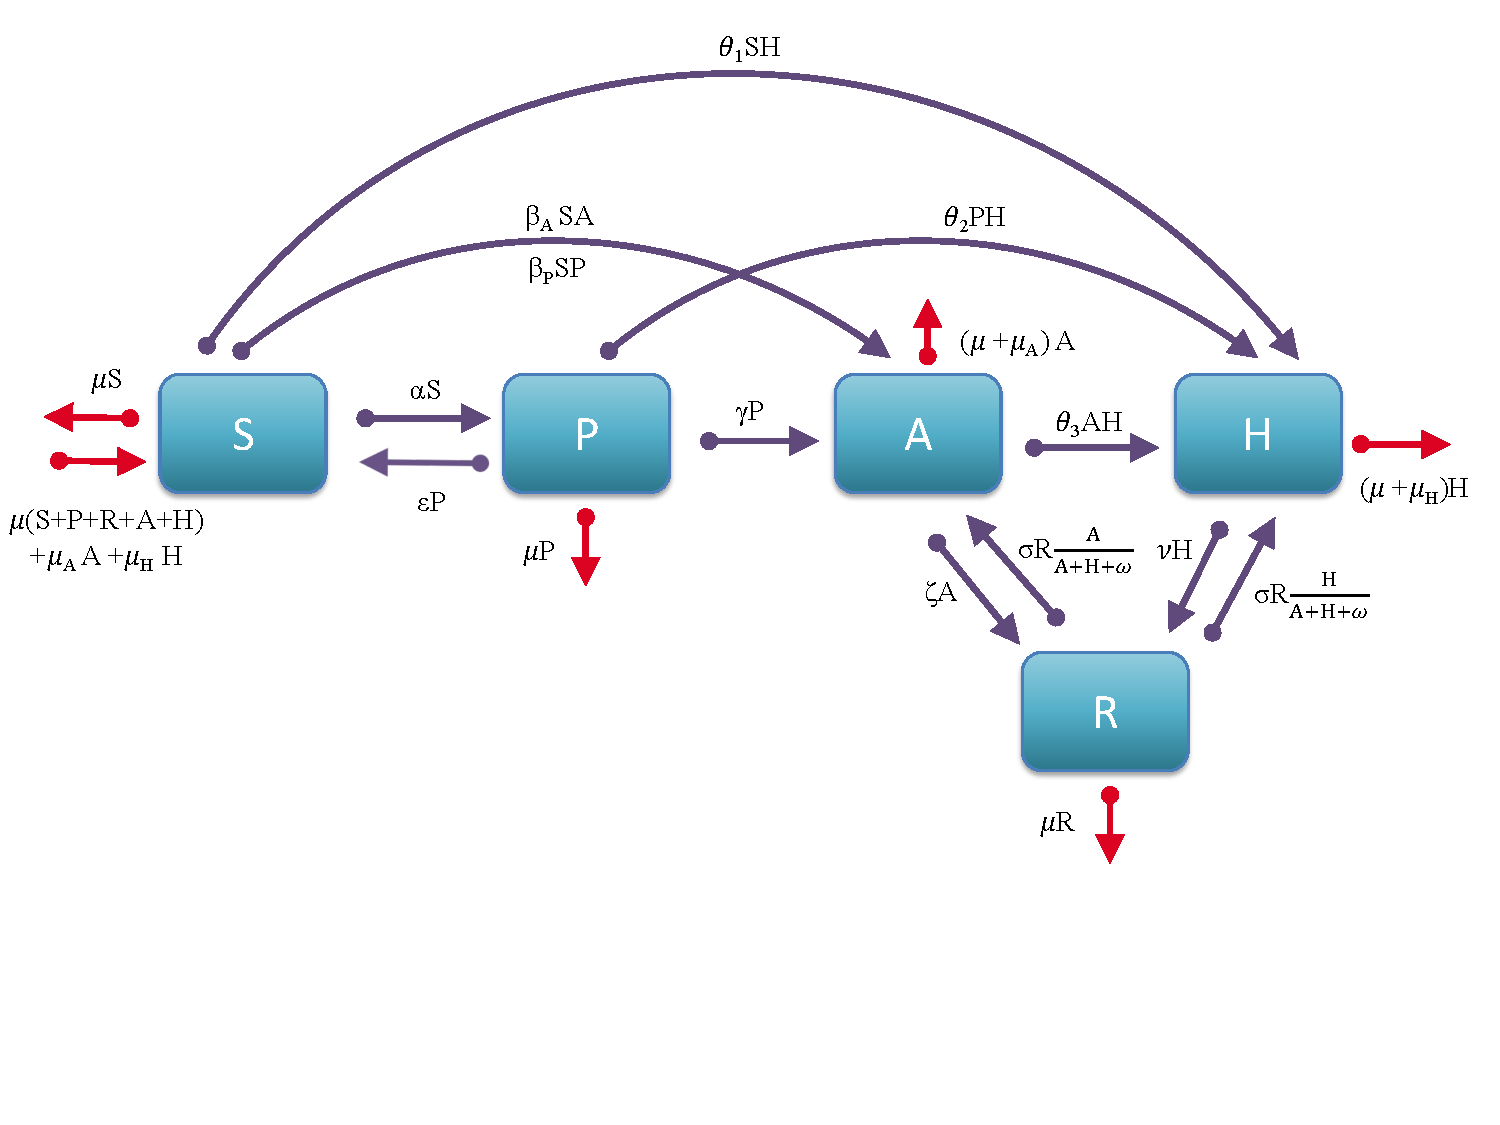
\includegraphics[scale=0.6]{heroin_schematic.pdf}
\vspace{-0.8cm}
\begin{center}
Figure 1: Schematic diagram for heroin model
\end{center}

%Christopher's words: (Regarding why we have so many assumptions). What can we say with a simple model? And from there, what can't we say? <-- This latter question gives us direction for how to improve the model and what we should do to build/extend the model further. 



%%%%%%%%%%%%%%%%%%%
%%%%%%%%%%%%%%%%%%%
%EXISTENCE OF ODE SOLUTION%
%%%%%%%%%%%%%%%%%%%
%%%%%%%%%%%%%%%%%%%

 \textbf{Proof of existence of solution to ODE system} \\
Will show existence of solution to my ODE system?




%%%%%%%%%%%%%%%%%%%
%%%%%%%%%%%%%%%%%%%
%NON-NEGATIVE IC => NON-NEGATIVE SOLUTIONS%
%%%%%%%%%%%%%%%%%%%
%%%%%%%%%%%%%%%%%%%



\textbf{Proof of non-negative initial conditions guaranteeing non-negative solutions} \\
We will now show that starting with non-negative initial conditions, solutions for the system (1)-(5) are guaranteed to be non-negative for all time, using the following theorem which is an adaptation of Theorem 2.1 in \cite{Smith}: 
 
 \textbf{Theorem 1} (\cite{Smith}: adapted version of Theorem 2.1, Chapter 5) 
\begin{comment} / Brittany Stephenson's dissertation 
\end{comment}
 \textit{Assume that when $\phi \in \mathbb{R}^n$ satisfies $\phi \geq 0$ with $\phi_{i}(0)=0$ for some $i$, then $f_i(\phi) \geq 0$. Then, if $\phi \in \mathbb{R}^n$ satisfies $\phi \geq 0$, the solution of $x'(t)=f(x(t)), x(t_{0})=\phi$ where $f: \mathbb{C}$ $\rightarrow$ $\mathbb{R}^n$ continuous, $\mathbb{C} \subset \mathbb{R}^n$ open and $\phi \in \mathbb{R}^n$, satisfies $x(t) \geq 0$ for all $t \geq t_{0}.$}
 
 \textbf{Proof} Consider the vector of initial conditions in $\mathbb{R}^5$, $\phi = (S_0, P_0, A_0, H_0, R_0).$ Since each vector component represents a proportion of a population, we know $\phi \geq 0.$ \\
 
1) Assume $\phi = (0, P_0, A_0, H_0, R_0) \geq 0.$ Then, 
\begin{center}
$f_1(\phi)=\epsilon P_0 + \mu (P_0+R_0)+(\mu + \mu_A) A_0 + (\mu+\mu_H) H_0 \geq 0,$
\end{center}
since all parameters and variables are non-negative. 
 
2) Assume $\phi = (S_0, 0, A_0, H_0, R_0) \geq 0.$ Then, 
\begin{center}
$f_2(\phi)=\alpha S_0 \geq 0,$
\end{center}
since $\alpha$ and $S_0$ are non-negative. 

3) Assume $\phi = (S_0, P_0, 0, H_0, R_0) \geq 0.$ Then,
\begin{center}
$f_3(\phi)=\gamma P_0 + \beta_{P} S_0 P_0 \geq 0,$
\end{center}
since all parameters and variables are non-negative. 
 
4) Assume $\phi = (S_0, P_0, A_0, 0, R_0) \geq 0.$ Then,
\begin{center}
$f_4(\phi)=0 \geq 0.$
\end{center}
 
5)  Assume $\phi = (S_0, P_0, A_0, H_0, 0) \geq 0.$ Finally,
\begin{center}
$f_5(\phi)=\zeta A_0 +\nu H_0 \geq 0,$
\end{center}
since all parameters and variables are non-negative. 

Thus, whenever $\phi \geq 0$ and $\phi_i(0)=0$ for some $i$, we see $f_i(\phi) \geq 0$. Therefore, since $\phi \geq 0$, then by Theorem 1, the solution $X(t)=(S(t), P(t), A(t), H(t), R(t)) \geq 0$ for all $t \geq 0$, as desired. $\square$



%%%%%%%%%%%%%%%%%%%
%%%%%%%%%%%%%%%%%%%
%PROOF OF BOUNDEDNESS%
%%%%%%%%%%%%%%%%%%%
%%%%%%%%%%%%%%%%%%%

 \textbf{Prove solution is uniformly bounded a priori}

 \textbf{Proof} We see $$\frac{dS}{dt} + \frac{dP}{dt} + \frac{dA}{dt} +\frac{dH}{dt} +\frac{dR}{dt} = 0$$
This means  $S(t) + P(t) + A(t) + H(t) +R(t) = c$ for some constant $c \geq 0$, upon integration with respect to time. Therefore, each state solution must be $\leq c$ for all $t \geq t_0$. Assuming we begin with non-negative initial conditions, then by previous work, we have shown that solutions will remain non-negative for all time. Thus, $0 \leq S(t), P(t), A(t), H(t), R(t) \leq c$ for all $t \geq t_0.$ As before, we set $c=1$, so that each of the state solutions represent a fraction of the population. In conclusion, our state solutions are uniformly bounded. $\square$
 
 \textcolor{blue}{Have checked if correct.}

 



%%%%%%%%%%%%%%%%%%%
%%%%%%%%%%%%%%%%%%%
%PROOF OF UNIQUENESS OF SOLUTION%
%%%%%%%%%%%%%%%%%%%
%%%%%%%%%%%%%%%%%%%



 \textbf{Proof of uniqueness of solution to ODE system} \\
\textcolor{red}{Fill in proof}. 




%%%%%%%%%%%%%%%%%%%
%%%%%%%%%%%%%%%%%%%
%DATA %
%%%%%%%%%%%%%%%%%%%
%%%%%%%%%%%%%%%%%%%




\textbf{Data} \\ \\
\textcolor{red}{Update from data\_collection.pdf}
We recognize that these estimated parameter values vary based on time and different locations within Tennessee, but are sufficient for analyzing the model. 
\begin{itemize}



\item The following are the \textbf{number of individuals in each class} for Tennessee in 2015: \\

*\textbf{Susceptibles}: (Total population in 2015-size of four other classes$=6,590,726-1,819,581-48,000-14,000-R_{0}=$FILL IN) \cite{USCensus} \\

*\textbf{Prescription opioid users}, 2015: 1,819,581 \cite{TNgov1} \\
Although this number does not explicitly state it is for individuals 12 and older, we assume it is since it comes from the Tennessee Department of Health; if it does include individuals under 12, we assume that number is negligible. \\

*\textbf{Opioid addicts}, 2015/2016 average for ``Pain Reliever Use Disorder" for individuals 12 and older: 48,000 \cite{NSDUH2} \\
We note that their definition of pain reliever use disorder includes those who meet the American Psychiatric Association criteria for dependence or abuse. Here, opioid dependence is classified as having "signs and symptoms that reflect compulsive, prolonged self-administration of opioid substances that are used for no legitimate medical purpose or...are used in doses that are greatly in excess of the amount needed for pain relief...regular patterns of compulsive drug use that daily activities are typically planned around obtaining and administering opioids." This definition falls under our definition of opioid addiction. Opioid abuse, on the other hand, they consider to be less severe than dependence, and would not lead to the development of withdrawal symptoms. This latter definition does not fall under our characterization of addiction, but we make a note of this to say that this estimate for those with a pain reliever use disorder may be overestimated for what we are concerned with, but is an acceptable approximation  \cite{DSM}.\\

*\textbf{Heroin/fentanyl addicts}, 2015/2016 average for ``Past Year Heroin Use" for individuals 12 and older: 14,000 \cite{NSDUH2}  \\ 
Although this number includes those who may have used heroin once or twice in the past year, we are under the assumption that the majority of these individuals are addicts and that very few, if any, individuals use heroin recreationally. In addition, the number of heroin users does not include fentanyl users explicitly, but we are under the assumption that those who take fentanyl are a subset of those who use heroin, and therefore, would mostly be included in these numbers. We admit the values may be slightly too low, for the cases of individuals who do fentanyl and not heroin, but data has not been found for fentanyl addicts only. Therefore, we are working under the assumption that it would be a negligible population that takes fentanyl without heroin. Overall, these two assumptions may work to balance one another out. 


%NSDUH Info for how do surveys for states: https://www.samhsa.gov/data/sites/default/files/NSDUHsaeMethodology2016/NSDUHsaeMethodology2016.pdf

\textit{*\textbf{Recovered addicts}: won't be able to find because we do not know the total number of individuals that have been in treatment, successfully finished, and not relapsed in our time frame}  \\



\item For Tennessee, the \textbf{total number of individuals taking prescription opioids} for pain \cite{TNgov1}: \\
2013: 1,845,144 \\
2014: 1,824,342 \\
2015: 1,819,581 \\
2016: 1,761,363 \\
2017: 1,636,374 

Although this number does not explicitly state it is for individuals 12 and older, we assume it is since it comes from the Tennessee Department of Health; if it does include individuals under 12, we assume that number is negligible. \\

\item For Tennessee individuals 12 and older, \textbf{the number of treatment admissions for non-heroin opiates/synthetics} as the primary substance of abuse to facilities that receive state/public funding (generally referring to funding by the state substance abuse agency) \cite{TEDS2015_SAMSHA_admissions}: \\
2005: 1,578 \\
2006: 1,529 \\
2007: 1,743 \\
2008: 2,022 \\
2009: 2,464 \\
2010: 3,384 \\
2011: 3,884 \\
2012: 4,203 \\
2013: 4,485 \\
2014: 4,530 \\
2015: 4,326 \\

We are under the assumption that if one were addicted to heroin in addition to prescription opioids, their heroin problem would be the primary reason for going to treatment and would be included in the following numbers. 

%can get "new arrivals to R" from this info, apparently: integrate dR/dt over time frame interested in (t_1 to t_2) and on RHS, integrate \zeta*A+\nu*H (or can break into two integrals on the RHS), and can get new arrivals; don't have to worry about double counting or people cycling \\

\item For Tennessee individuals 12 and older, \textbf{the number of treatment admissions for heroin} as the primary substance of abuse to facilities that receive state/public funding (generally referring to funding by the state substance abuse agency) \cite{TEDS2015_SAMSHA_admissions}: \\
2010: 199\\
2011: 240 \\
2012: 390 \\
2013: 555 \\
2014: 743 \\
2015: 1,083 \\


Again, these numbers do not include fentanyl users explicitly, but we are under the assumption that those who take fentanyl are a subset of those who use heroin, and therefore, would mostly be included in these numbers. We admit the values may be slightly too low, for the cases of individuals who do go to treatment with the primary substance of abuse being fentanyl, but there is not data available for those numbers currently. 


%All TEDS tables: https://wwwdasis.samhsa.gov/dasis2/teds.htm

\item We use data on the number of prescription opioid overdose deaths which include natural, semi-synthetic, and synthetic opioids; however, we subtract out the number of fentanyl overdoses (fentanyl is classified as a synthetic prescription opioid), since those overdoses are counted for in their own category, listed below. This results in the following  \textbf{total number of prescription opioid overdose deaths} \cite{PDO}: \\
2013:(637-53=) 584 \\
2014: (697-69=) 628 \\
2015: (848-169=) 679 \\
2016: (1,009-294=) 715 \\

Although this number does not explicitly state it is for individuals 12 and older, we assume it is since it comes from the Tennessee Department of Health; if it does include individuals under 12, we assume that number is negligible. \\

item We add together the heroin and fentanyl overdoses from the years 2013-2016 for the state of Tennessee. The \textbf{total number of heroin and fentanyl overdoses} for these four years are: \\
2013: (63+53=) 116 \\
2014: (147+69=) 216 \\
2015: (205+169=) 374 \\
2016: (260+294=) 554 \cite{PDO}. 

Although this number does not explicitly state it is for individuals 12 and older, we assume it is since it comes from the Tennessee Department of Health; if it does include individuals under 12, we assume that number is negligible. \\


%SEE WORK on 11/19/18 meeting notes for mu_A, mu_H, mu
We may calculate the overdose death rate in the year 2015, since we know the number of addicted individuals in that year. To find the continuous-time rate at which individuals are dying from the addicted class, we consider the equation $k A_{0}=A_{0}e^{-\mu_{A}t}$, where $A_0$ is the number of individuals addicted to opioids in 2015 and $k$ is the proportion of these individuals in the addicted class at the start of 2016 (when $t=1$). In 2015, there were 679 individuals out of the entire Tennessee population 12 and older that overdosed on prescription opioids \cite{PDO}. However, it is estimated that only 54.6\% of these individuals were actually at an increased risk for an opioid-related overdose death; we will assume that if an individual met the criteria for at least one high-risk factor, that they were considered addicted to opioids \cite{Gwira}. Therefore, we will assume 54.6\% of the 679 individuals that overdosed were addicted. With a total of 48,000 opioid addicts in 2015, this means that (48,000-0.546$\cdot$679)/48,000 $\approx$ 0.992 is the proportion of addicted individuals that remain by the beginning of the next year. This implies 0.992$A_0=A_0 e^{-\mu_{A}(1)}$, and solving results in $\mu_{A} \approx 0.00775.$

Similarly, we may calculate $\mu_{H}$. There were 14,000 heroin/fentanyl addicts in 2015 and 374 heroin-related overdoses. We make the assumption that if an individual died of a heroin overdose they were addicted in line with our previous assumptions that if one is using heroin, they are considered addicted due to the nature of the drug. This means that (14,000-374)/14,000 $\approx$ 0.973 is the proportion of heroin users that remain at $t=1$, which implies 0.973$H_0=H_0 e^{-\mu_{H}(1)}$, which results in $\mu_{H}$ $\approx 0.0271$, the continuous-time rate at which individuals are dying from the heroin class.

%we view it as a good thing that methadone was pulled out separately from this data for overdoses, because it's used in treatment in order to reduce cravings and not necessarily supply the high 

\item We make a note that individuals that do not have an opioid use disorder and die because of an opioid overdose are counted in the ``natural mortality rate." 


%Could use overdose data of heroin compared to number of heroin addicts in order to get a scaling, and then be able to determine number of fentanyl addicts based on the number of fentanyl overdoses. But for now, going with subset argument, that heroin users includes fentanyl users. 


\item Total population estimated in Tennessee each year \cite{USCensus}: \\
2013: 6,490,795 \\
2014: 6,540,007 \\
2015: 6,590,726 \\
2016: 6,649,404 \\
2017: 6,715,984 \\
\textcolor{red}{2018: FILL IN} \\

There was an estimated 1,073,214 individuals Tennessee in 2018 aged 12 and under. To figure out those who are 12 years old, we take approximately 1/8th of the individuals that are in the age group 5-12, which is approximately 83,175 individuals \cite{DOHHS}. Thus, an estimated 990,039 individuals are \emph{under} the age of 12 in Tennessee. Given the last total population estimate for 2017 being 6,715,984 from above, this means that approximately 15\% of the population is under the age of 12. \textcolor{red}{FIX when get updated 2018 total population}. Since we do not see a reason for this percentage to be significantly different from year to year, we assume that this percentage is constant throughout the time period we are looking at. Then, we are able to consider the following \textbf{Tennessee population estimates for individuals 12 and older} in order to align with the rest of the data that is in this age range by taking off 15\% of the above total population estimates.  \\
2013: 5,517,176 \\
2014: 5,559,006 \\
2015: 5,602,117 \\
2016: 5,651,993 \\
2017: 5,708,586 \\

%Could be helpful if need for individuals under 12: https://factfinder.census.gov/faces/tableservices/jsf/pages/productview.xhtml?src=CF 
\item The \textbf{age-adjusted death rate} for Tennessee in 2016 was calculated to be 886.3 out of 100,000 individuals, or approximately 50,094 people out of a total population 12 and older of 5,651,993 \cite{Kaiser}. Subtracting off the number of people who died from a prescription opioid or heroin/fentanyl overdose in 2016 results in 48,825 people who died that year. This implies that (5,651,993-48,825)/5,651,993 $\approx$ 0.991 is the proportion of the population that remains by the beginning of 2017. If we consider $T_0$ to be the total population in 2016, we can find the continuous-time rate at which individuals die naturally from the equation 0.991$T_0$=$T_0e^{-\mu t}$, which results in the natural death rate $\mu \approx 0.00868$.



\item \textbf{Relationship among $\theta_1$, $\theta_2$, and $\theta_3$:} Since we could not find data for values of $\theta_1$, $\theta_2$, or $\theta_3$ for Tennessee, we consider a national study of individuals 12 and older to establish a relationship among these three rates. For a national study consisting of 609,000 participants, ``the recent heroin incidence rate was 19 times higher among those who reported prior non-medical pain reliever (NMPR) use (0.39\%) than among those who did not report NMPR use (0.02\%) \cite{Muhuri}.
Thus, we will extrapolate this information to say that the rate that prescription opioid users and opioid addicts move to heroin use is 19 times greater than the rate at which susceptibles move to heroin use (i.e. $\theta_2 + \theta_3$ $>$ 19$\theta_1$). Although $\theta_2$ is going from P to H and consists of prescription opioid users who do not misuse their prescription, we will make the assumption that those who misuse are much more likely to be the ones to move to heroin use. \\
\pagebreak

\textcolor{red}{\emph{Ignore for now, later tell story about what model tells us regarding this.}} \\
\textbf{Information for moving from recovery to opioid addiction or heroin/fentanyl addiction, $\sigma_A$ and $\sigma_H$:} 

We consider here the number of individuals in Tennessee age 12 and older who dropped out of treatment and assume that dropping out would result in an individual going back into addiction since they did not successfully complete treatment. The number of drop-outs from medication-assisted opioid detox programs and outpatient medication-assisted opioid programs was reported as essentially zero for Tennessee in 2012, 2013, and 2015, and 3 or fewer for 2011 and 2014, which does not seem realistic \cite{TEDS2011_SAMSHA_discharges, TEDS2012_SAMSHA_discharges, TEDS2013_SAMSHA_discharges, TEDS2014_SAMSHA_discharges, TEDS2015_SAMSHA_discharges}. Therefore, to get an estimate for what this value may look like, we took the total number of admissions into all drug treatment programs for each year and calculated the drop-out rates for each of those years: \\
2011: 2,910/13,422=.217  \cite{TEDS2011_SAMSHA_admissions,TEDS2011_SAMSHA_discharges} \\
2012: 3,127/13,525=.231 \cite{TEDS2012_SAMSHA_admissions, TEDS2012_SAMSHA_discharges} \\
2013: 3,273/14,476=.226 \cite{TEDS2013_SAMSHA_admissions, TEDS2013_SAMSHA_discharges} \\
2014: 3,164/14,909=.212  \cite{TEDS2014_SAMSHA_admissions, TEDS2014_SAMSHA_discharges} \\
2015:  3,039/14,916=.204 \cite{TEDS2015_SAMSHA_admissions, TEDS2015_SAMSHA_discharges} \\

We take the average of these drop out rates and extrapolate this to be an estimate for those dropping out of opioid-related therapies: .218. (SEEMS WAY TOO LOW).

%Additional treatment admissions data for Tennessee: https://wwwdasis.samhsa.gov/dasis2/teds_pubs/2015_teds_rpt_st.pdf


\end{itemize}


\textcolor{red}{Things to investigate for TN: Pilfering Prevention Act in TN: lockable pill bottles with code to unlock; opioid supply limit policy; STOPTN organization to look into} 


%%%%%%%%%%%%%%%%%%%
%%%%%%%%%%%%%%%%%%%
%PARAMETER ESTIMATION%
%%%%%%%%%%%%%%%%%%%
%%%%%%%%%%%%%%%%%%%



\textbf{Parameter Estimation} \\
%May use ordinary least squares or bayseian inference since we are hoping to have data from experts
%If do Bayes: see notes from 11/28/17 meeting 
%epsilon for Christopher's opioid paper from 0.8 to 8 because of units and t is a year 
\textcolor{red}{Fill in details about OLS basics and work for my model.}

In order to estimate parameters for our model, we use data from above and compared it to the proportions of the population in the classes at in certain years or the proportion of the population that entered the classes in certain years (go into specifics depending on what use). We utilized the ordinary least squares method and formulated an objective function to minimize, which consists of the squared differences between the data and model simulations. We used the optimization toolbox in MATLAB and specifically utilized the MultiStart algorithm and fmincon and used FILL IN as the number of starting points to ensure that the global minimum is found, as this is a local solver. \textcolor{red}{Write about what fmincon uses (gradient?) and know more about how it works at least for defense.} \\

\textcolor{red}{Do plots later once parameters set.}



%%%%%%%%%%%%%%%%%%%
%%%%%%%%%%%%%%%%%%%
%ADDICTION-FREE EQUILIBRIUM%
%%%%%%%%%%%%%%%%%%%
%%%%%%%%%%%%%%%%%%%



 \textbf{Addiction-Free Equilibrium} 
\textcolor{red}{DO UPDATE FROM NEW MODEL Was unable to solve for endemic equilibrium (in binder with date 4/10/18)...need to eventually or just prove existence of one? Bifuraction analysis?}

To find the addiction-free equilibrium, we set equations (1)-(5) equal to zero and require that $A=H=R=0$ since these three compartments consist of individuals who are addicted to opioids or heroin. We are left with the system: \\
\[0=-\alpha S^* -\beta_{P} S^* P^* + \epsilon P^* +\mu P^* \quad\]
\[0=\alpha S^* - \epsilon P^* -\gamma P^* - \mu P^* \quad\]
\[0=\gamma P^* + \beta_{P} S^* P^*.   \quad\]



If $P^*=0$, then the only solution is $S^*=P^*=H^*=R^*=0$, but $S^*=P^*=H^*=R^*=1$ by assumption, so this is not possible. Thus, we will assume $P^* \neq 0. $ This forces $\gamma + \beta_{P} S^* =0$ and since all of our parameters and variables are non-negative, then it must be $\gamma=0$ and $\beta_{P}=0$. We have that $\gamma=0$ means that individuals who are prescribed opioids cannot become addicted to opioids, and $\beta_{P}=0$ means that only black market opioids are available for susceptibles to become addicted to opioids and there are no excess prescription drugs available. Under the assumption that $\gamma=0=\beta_{P}$ to ensure the existence of our addiction-free equilibrium and that $1=S+P+A+H+R$, we calculate the addiction-free equilibrium to be: \\

\[S^*=\frac{\epsilon + \mu}{\alpha + \epsilon +\mu}\quad\]
\[P^*=\frac{\alpha}{\alpha + \epsilon +\mu}\quad\]
\[A^*=0\quad\]
\[H^*=0\quad\]
\[R^*=0\quad\] 

Note that enforcing $P^* \neq 0$ implies that $\alpha \neq 0$, as well, which means that individuals are still able to be prescribed opioids. 

%Lenhart says won't do bifurcation analysis for this paper 


%%%%%%%%%%%%%%%%%%%
%%%%%%%%%%%%%%%%%%%
%BASIC REPRODUCTION NUMBER%
%%%%%%%%%%%%%%%%%%%
%%%%%%%%%%%%%%%%%%%


\textbf{Basic Reproduction Number, \textbf{$\mathscr{R}_0$}} \\
\textcolor{red}{DO UPDATE FOR NEW MODEL Re-check work in future because removed delta, but should be same final result except 
delta is not a part of "c." In addition, changed notation from $\beta$ and $\xi$ to $\beta_{A}$ and $\beta_{P}$, so make sure all notation was correctly converted.} \\
%Can numerically check R_0 (i.e. plug in specific values for F and V and make sure that matches my R_0). Make sure if R_0>1, goes away from my equilibrium and if R_0<1, goes toward my equilibrium. 

The basic reproduction number, denoted $\mathscr{R}_0$, is a term used in epidemiological models that gives the expected number of secondary disease cases that result from the introduction of a disease to a susceptible population. The value of $\mathscr{R}_0$ represents how successful the spread of the disease is expected to be; if $\mathscr{R}_0 < 1$, then the disease is expected to die out and the disease-free equilibrium will be locally stable; conversely, if $\mathscr{R}_0 >1$, then the disease is expected to spread and the disease-free equilibrium will be unstable \cite{Driessche}. \\ \\
 This idea may be applied to the context of our model since for the addiction-free equilibrium to occur, $\gamma$ and $\beta_{P}$ must both be equal to 0, which means individuals can become addicted only with interactions with opioid addicted individuals or heroin users so this takes the form of an infectious disease. Thus, in this case in which the prescription part is essentially taken out of the model so that it is a black-market-only driven model, $\mathscr{R}_0$ can be calculated. This value will be the ratio of the number of new addictions in the next year compared to the current year. At the addiction-free equilibrium, the population is completely susceptible, as needed for $\mathscr{R}_0$ to be an accurate measurement of addiction potential. 
We note that our goal in this section is to explore the structure of the model and not obtain a result for the full model. The disease compartments are those that contain infected individuals, or in our case, addicts \cite{Driessche}. Our model incorporates three addiction compartments, A, H, and R, since these all consist of opioid and/or heroin addicted individuals. We will utilize the Next Generation Matrix Method in order to calculate $\mathscr{R}_0$.


For the purposes of calculating $\mathscr{R}_0$, we will assume $\gamma =0$ and $\beta_{P} =0$ in order to ensure the existence of the addiction-free equilibrium. This results in the following system:
\[\dv{S}{t} = -\alpha S - \beta_{A} SA  - \theta_{1} SH +\epsilon P +\mu (P+R) + (\mu+\mu_{A})A + (\mu+\mu_{H}) H \quad \] 
\[\dv{P}{t} = \alpha S - \epsilon P  - \theta_{2}PH- \mu P    \quad\]
\[\dv{A}{t} = \sigma_{A} R +\beta_{A} SA  -\zeta A - \theta_{3}AH-(\mu + \mu_{A})A   \quad\]
\[\dv{H}{t} = \theta_{1}SH+\theta_{2}PH+\theta_{3}AH + \sigma_{H}R-\nu H-(\mu+\mu_{H})H  \quad\]
\[\dv{R}{t} = \zeta A +\nu H -\sigma_{A}R-\sigma_{H}R -\mu R.\quad\]


In general, the differential equations of the $n$ disease compartments, $x_i'$, may be written as: 

\[{x_i'} = \mathscr{F}_{i} (x,y)-\mathscr{V}_i (x,y),\quad i=1,...,n\] 

where $x$ is a vector with the disease compartments as components, $y$ a vector with the non-disease compartments as components, $\mathscr{F}_{i}$ represents the rate that secondary infections contribute to disease compartment $i$ and $\mathscr{V}_{i}$ represents the rate of transitions, i.e. rate at which the disease compartment $i$ is decreased by means of death, recovery and progression of the disease for $i=1,2,3$ \cite{Driessche}. 

Thus, for our three addicted compartments, we may write: 

$$\dfrac{dA}{dt} = \mathscr{F}_{1} (x,y)-\mathscr{V}_{1}(x,y)$$
$$\dfrac{dH}{dt} = \mathscr{F}_{2} (x,y)-\mathscr{V}_{2}(x,y)$$
$$\dfrac{dR}{dt} = \mathscr{F}_{3} (x,y)-\mathscr{V}_{3}(x,y),$$

where $x= {[A\quad H\quad R]}^{T}$ and $y= {[S\quad P]}^{T}$.



Thus, under the assumption that A, H and R are the addicted compartments and abiding by the parameter restrictions stated above, the assumptions of the Next Generation Method are satisfied for matrices $\mathscr{F}$ and $\mathscr{V}$ formulated here:

\begin{center}
$\mathscr{F}=$
$ \begin{pmatrix}

\beta_{A} SA \\
\theta_{1}SH+\theta_{2}PH \\
0
\end{pmatrix}$



$\mathscr{V}=$
$ \begin{pmatrix}

-\sigma_{A}R+\zeta A+\theta_{3} AH + (\mu +\mu_{A})A \\
-\theta_{3}AH-\sigma_{H}R+\nu H +(\mu +\mu_{H}) H \\
-\zeta A -\nu H +\sigma_{A}R +\sigma_{H}R +\mu R\\
\end{pmatrix}$.
\end{center}

These assumptions include the following: 
\begin{itemize}
\item $\mathscr{F}_{i} (0,y)=0$ and $\mathscr{V}_{i}(0,y)=0$,  $\forall$$y \geq 0$, $i=1,2,3$, which ensures that new addictions arise only from interacting with those currently addicted, and there is no immigration into the addicted compartments; these guarantee that the population free of addiction remains that way. 
\item $\mathscr{F}_{i} (x,y) \geq 0$, $\forall$$x,y \geq 0$, $i=1,2,3$ since these represent new addictions. 
\item $\mathscr{V}_{i}(x,y) \leq 0$ whenever $x_i=0, i=1,2,3$ since there must be inflow only when the respective compartment is empty. 
\item $\sum_{n=1}^{3} \mathscr{V}_{i}(x,y) \geq 0$, $\forall x,y \geq 0$ since this represents the total outflow from all addicted compartments. 
\item The addiction-free system, $\dv{S}{t}\bigg|_{A,H,R=0}$ and $\dv{P}{t}\bigg|_{A,H,R=0}$ has a unique equilibrium, ($\frac{\epsilon+\mu}{\alpha+\epsilon+\mu}$,$\frac{\alpha}{\alpha+\epsilon+\mu}$) that is asymptotically stable. 
\end{itemize}

Taking $F=\frac{\partial \mathscr{F}_i}{\partial x_j} (0, y_0)$ and $V=\frac{\partial \mathscr{V}_i}{\partial x_j} (0, y_0)$, $i, j =1, 2, 3$, where (0, $y_{0}$) $=(\frac{\epsilon + \mu}{\alpha + \epsilon +\mu},\frac{\alpha}{\alpha + \epsilon +\mu},0,0,0)$ is the addiction-free equilibrium, we calculated the following \cite{Driessche}: 



\begin{center}
$F=$
$ \begin{pmatrix}

\beta_{A} S^* &  0  & 0 \\
0 & \theta_1 S^* +\theta_2 P^* & 0\\
0  &   0 & 0\\
\end{pmatrix}$



$V=$
$ \begin{pmatrix}

\zeta +\mu +\mu_A &  0  & -\sigma_A \\
0 &  \nu+\mu+\mu_H & -\sigma_H\\
-\zeta& -\nu  & \sigma_A + \sigma_H + \mu\\

\end{pmatrix}$.
\end{center}

The eigenvalues of $FV^{-1}$ are calculated to be: 
\begin{center}
$\sigma (FV^{-1}) = \{0, \frac{(r+s)-\sqrt{(r-s)^2+4\beta_{A} S^* z  \sigma_A \zeta \sigma_H \nu}}{2det(V)} 
, \frac{(r+s)+\sqrt{(r-s)^2+4\beta_{A} S^* z  \sigma_A \zeta \sigma_H \nu}}{2det(V)} 
\}$
\end{center}

where $a=\zeta +\mu + \mu_A$, $b=\nu + \mu + \mu_H$, $c= \sigma_A + \sigma_H +\mu$, $z=\theta_1 S^* + \theta_2 P^*$, $ r=\beta_{A} S^* (bc-\sigma_H \nu), s=z(ac-\sigma_{A} \zeta)$, and $det(V)=a(bc-\sigma_H\nu)-\sigma_A\zeta b$.

$\mathscr{R}_0$ may then be determined as the spectral radius of $FV^{-1}$, in which the $(i,j)$ entry is the expected number of secondary addictions in compartment $i$ produced by individuals initially in compartment $j$ :
\begin{center}
$\mathscr{R}_0=$ $\frac{(r+s)+\sqrt{(r-s)^2+4\beta_{A} S^* z  \sigma_A \zeta \sigma_H \nu}}{2det(V)}. $
\end{center}

This value is the spectral radius since it is the largest eigenvalue greater than 0. We can see this by first noting that the radicand $(r-s)^2+4\beta_{A} S^* z  \sigma_{A} \zeta \sigma_{H} \nu$ is positive, since all parameters are positive. In addition, $r$ is positive because in the multiplication of $bc=\ \mu^{2} + \mu \nu+ \mu \mu_{H} + \mu \sigma_{A} + \mu \sigma_{H}+ \nu \sigma_{A}+$ \hl{$ \sigma_{H} \nu $} $+ \mu_{H}\sigma_{A}+\mu_{H}\sigma_{H}$, all terms are positive and the highlighted term cancels with $-\sigma_{H} \nu$, leaving only a positive sum. Multiplying by $\beta_{A} S^*$, the resulting value $r$ is positive. Similarly, $s$ is positive because in the multiplication of $ac= \mu_{A} \mu+ \mu_{A} \sigma_{A}+\mu_{A} \sigma_{H} +\mu^{2} +\mu \zeta+ \mu \sigma_{A}+\mu \sigma_{H}+$ \hl{$\sigma_{A} \zeta$} $+ \zeta \sigma_{H}$, all terms are positive and the highlighted term cancels with $-\sigma_{A} \zeta$, again resulting in a sum of only positive terms. Multiplied against positive value $z$, this results in $s$ being positive. Finally, the expansion of $det(V)$ is positive. This is because $bc$ is a positive sum containing a term that cancels with $-\sigma_{H} \nu$ as described above and $ac$ shown above contains the term $\sigma_{A} \zeta$ which multiplied with b cancels with $-\sigma_A\zeta b,$ thus resulting in a positive determinant. \textcolor{red}{Need to prove AFE is stable if $\mathscr{R}_0$ $<$ 1 and unstable if $>$ 1?}

%Don't include, most likely: Increasing $\beta_{A}$ (the rate of addiction via non-prescription means), $\theta_1$ (the rate of heroin addiction of the susceptible population), and $\theta_2$ (the rate of heroin addiction of the prescribed population), all increase $\mathscr{R}_0$ since these parameters only appear in the numerator of $\mathscr{R}_0$, specifically within the $r$, $z$, and $s$ terms. \\ 






%%%%%%%%%%%%%%%%%%%
%%%%%%%%%%%%%%%%%%%
%SENSITIVITY ANALYSIS%
%%%%%%%%%%%%%%%%%%%
%%%%%%%%%%%%%%%%%%%



\textbf{Sensitivity Analysis} 
%Maybe use Brain Dynamics Toolbox for heat maps? https://github.com/breakspear/bdtoolkit
%second order rates (like parameter*S*H) won't have much sensitivity, something to look out for 
\textcolor{red}{Latin Hypercube/ PRCC or Sobol or both? Do we need local sensitivity analysis at all?} \\
\textcolor{red}{Things to do: Write up Marino paper basics of Latin Hypercube/PRCC sensitivity analysis; alter LHS/PRCC code sent from Christina (talk with her about which codes need to be changed/not be changed...see Lenhart seminar notes from sensitivity analysis meeting, as well); finish writing up Sobol basics; alter Sobol code (remove $\delta$)} 
%Info: https://www.mathworks.com/help/sldo/ug/what-is-sensitivity-analysis.html , https://www.mathworks.com/help/sldo/ug/sampling-parameters-and-states.html  
%Variance methods: how big sample space affects results?
\textcolor{red}{Will need to be updated:} In order to explore the sensitivity of each of the population classes to each of the parameters, we implemented Sobol sensitivity analysis in which the Saltelli sampler is utilized to generate N(2D+2) parameter samples where N$=$FILL IN is the number of sample points and D=16, the number of parameters in the model for a total of FILL IN samples \cite{Herman}. 
Saltelli are the statistically good points chosen in the parameter space to test and records S, P, A, H and R at the final time (t=10 years) for the parameter choices. Samples N points from the problem and returns a matrix of parameter values. 
%Think about why N(2D+2) and why N(D+2) for taking out second order interactions. 
\textcolor{red}{Look into total order indices: total variance (sum?), expectation (variance), normalized sum. Look at Saltelli reference, equation 44: term+complement+interaction terms} \\
\textcolor{red}{Once have baseline parameters, do +/- 50\% for each parameter and cut off $\mu$ so does not go all the way to 0?}
Both $\mu_{A}$ and $\mu_{H}$ were restricted to the domain $[0,0.1]$ with the remaining parameters ranging on the entire domain $[0,1]$. For first-order indices, only one parameter is varied and the rest are held constant; for second-order indices, two parameters are varied and the rest are held constant; and for total-order indices, every combination of parameters is varied, from a single parameter varying alone to all higher-order interactions between parameters. The length of the colored bars, with each color representing a specific class, measures the contribution of a certain parameter to the variance of each of the classes in the model. The longer the colored bar, the higher the effect the parameter has on that class of individuals; the sum of each color adds to 1, so that for each parameter, the relative contribution to each of the classes is represented. We are able to retrieve the confidence intervals on the sensitivity of each of the populations to a respective change in the parameter(s) for first order changes, second order changes and total order changes. \\
\textcolor{red}{Change time step to -1: result[0][-1] I believe, because want to see how outputs (S,P,A,H,R) are affected at the FINAL time}

%Add in sensitivity analysis results and confidence interval information once converges 
%Takes the mean from the last 100 (or 10 for the case of t=10) time steps. (I thought final time??) \\
%Total --take average of all interactions for plots?? \\
%Need to scale sensitivities of muA and muH based on their domain $[0,0.1]$??

%Per Lenhart--use sensitivity analysis results to parse out different pieces of information; such as integrate \alphaP to get all new addiction individuals??
\pagebreak



%%%%%%%%%%%%%%%%%%%
%%%%%%%%%%%%%%%%%%%
%FUTURE WORK/IDEAS%
%%%%%%%%%%%%%%%%%%%
%%%%%%%%%%%%%%%%%%%




\textbf{Future Work/Ideas} \\
-Obtain local data from Knox County/East Tennessee, can calculate $\mathscr{R}_0$ from there (would expect $<$ 1 b/c prescriptions seem to be a huge driving force behind addiction to opioids and individuals switching to heroin use. Contact with Davide Stern (UT hospital), Paul Erwin, Agricola Odoi, Kelly Cooper\\
-Perform sensitivity analysis to determine the sensitivity of each of the classes to the parameters (i.e. the contribution of each of the parameters to the sizes of the classes). Plan to use Sobol sensitivity analysis in which the saltelli sampler is utilized to generate (statistically good) parameter samples. Will only perform on the full  odel, not the AFE b/c that would require $t$ very large and we want to look at shorter term, such as $t=10$ years. Will perform first, second and total indices. \\
-Fit parameters to data that are difficult to find in literature. \\
-Explore management strategies for how to best treat pain with prescriptions while reducing opioid addiction and heroin use (optimal control or scenario analysis: if reduce parameter, what happens).  \\
Possible extentions: \\
-Break recovery class into two different classes for opioid addicts and heroin users (look at pain management and why people relapse: START paper and Addiction Treatment Study). \\
-Look into gender, race, socioeconomic class, incarceration, or rural versus urban location to investigate differences; treatment programs/types of treatment/success rates (see Modeling Gender Differences in Drug Abuse Epidemics paper, paper copy in desk and Length of Stay in Different Drug Using States: Lifestyles of Problem and Recreational Drug Consumers for location, also see "future papers to read" in heroin folder)
-Significance of naloxone for reversing effects of overdose 
-Consider Markov Chain model (Lou from oral exam) 
-Linda Allen slides from Stochastic Modeling of Biological and Ecological Systems 2018 MN workshop 
-Incarceration 
-Different treatment programs/successes 
%maybe answer if the 5-day of 3-day limit to initial opioid prescriptions is good or not 

For a paper: \textit{Acknowledgements: The authors would like to thank Dr. Nicholas Battista and Leigh Pearcy for their contributions.}


%%%%%%%%%%%%%%%%%%%
%%%%%%%%%%%%%%%%%%%
%DISCUSSIONS WE'VE HAD/THOUGHTS%
%%%%%%%%%%%%%%%%%%%
%%%%%%%%%%%%%%%%%%%



\textbf{Discussions we've had/thoughts} \\
-For past drug waves: when did the media begin to care about the drug and its effects on society? Maybe incorporate feedback effect ( maybe functional form for terms going to addiction or heroin, etc.?) based on how the media/information available to the public affects the behavior of people and therefore the proportions of A and H (i.e. maybe our form now is good for the beginning but then may need to be altered as time goes on).\\
-There is a spectrum between P and A; maybe include a bucket for prescription misusers? May be difficult with data because questions may ask: ``have you misused prescription opioids in the past 12 months" and if someone has one time, they say "yes" but it's not an ongoing thing...so that's why we stick with addicteds only. Although there may be "misusers" in recovery, we assume that someone would not be in recovery unless they are actually addicted (i.e. harmful/interfering in their lives), so maybe people don't like to admit they are addicted, for example.\\
-Consider relapse again in future-it's hard to keep track of how people got to recovered in the first place (from A or from H), so for now, doing $\sigma_A$ and $\sigma_H$ linear rates for relapse--may need to change in future. Later, may split into $R_A$ and $R_H$ to keep them separate...first want to see if ``catchall" R or $R_A$ and $R_H$ even matter to the dynamics?\\
-May look into ``targeted reproduction number" (simpler representation of $\mathscr{R}_0$), or ``type reproduction number", or breaking into cycles (if look at certain cycle, what would $\mathscr{R}_0$ be)\\
-Reconsider PH and SH pathways? \\
-Gabapentin mixed with opioids, instead of fentanyl \\
-Medical doctors concerns are about how to prescribe, need a good policy; are they more focused on alpha or epsilon? Does media affect doctors? 
-Variance of length in P hard to put in ODE model \\
\\ \\

People: Met with Kelly Cooper, Laurie Meschke, Clea McNeely, Matthew Harris, Sharon Davis, Wil Cantrell; Future connections?: Dr. Steve Loyd at TN Substance Abuse Services; Hughes Melton from Virginia Dept of Behavioral Health and Developmental Services (through Wil Cantrell, see email 12/1/18); Chris McCurty at the Florida Center for Excellence; Don Burke at University of Pittsburgh; Charles Simms from Economics dept at UT;  Dr. Bruce Ramshaw, Department of Surgery at UT Medical Center and UT Graduate School of Medicine (seems that he would be able to provide information specifically about opioid prescriptions post-surgery); (See email: medical doctors to contact? on 10/8/2018 for next three people) Dr. Daniel Sumrok, Center of Addiction Science at UT Health Science Center in Memphis (a few important quotes from website article suggest we could potentially get information on how doctors are changing their prescribing behaviors: ``The picture of addiction is much different now than it was even a decade ago. Anyone can become addicted to painkillers, and we are doing our part to reduce that dependency rate" and ``Center for Addiction Science trains physicians and health care professionals in evidence-based protocols to better recognize, diagnose, treat and prevent addiction."); Dr. Stephanie Vanterpool and Dr. Jason Buehler regarding opioid alternatives for surgery 
\\ \\

Optimal control: \\
-functional consider expense of effort and cost of addiction from prescriptions? \\
-time-varying controls to move people from class to class with money (i.e. into recovery) \\
-add control to rates going between R and A or H (i.e. zeta, nu, $sigma_A$, $sigma_H$) or going to P from S (i.e. alpha) or going to S from P (i.e. epsilon or gamma) with spending money or with some amount of effort in terms of money and make as a function of years such as alpha(t) or epsilon(t) \\
-what can you affect by spending money on the problem? People going into/out of recovery? Identify those who are addicted/contact and trace people? \\
-P to A transition, some due to lack of doctor awareness? \\


 



 




\pagebreak

\bibliography{HeroinModel}

 \end{document}
